\emph{Artificial neural networks} or simply \emph{neural networks} are one of the most popular nonlinear classifiers. Although initially inspired in the way biological neurons integrate information~\cite{McCulloch1943, Widrow1960, Rosenblatt1962}, they evolved to specialize in nonlinear modelling at the expense of biological adherence~\cite{Rumelhart1986}.% We discuss here multilayer feedforward neural networks, the name should become obvious after a few paragraphs.

\emph{Multilayer feedforward neural networks} are composed of $L$ layers of \emph{neurons}, the computation units.% Each unit is connected to every unit in the previous and next layer.
%[[; units in a layer are|, ] [fully] connected to [every] units in|. Each layer is fully connected to] the previous and next layer (except for [units in] the first and last layer
The first layer, called the \emph{input layer}, has $s^{(1)} = n$ units and receives the feature vector $x \in \mathbb{R}^n$ while the last layer or \emph{output layer} has $s^{(L)} = K$ units corresponding to the $K$ possible classes. Every other layer is called a \emph{hidden layer} (Fig.~\ref{fig:NeuralNetwork}). The neural network receives an input $x \in \mathbb{R}^n$, processes it layer by layer and outputs a vector $h_\Theta(x) \in \mathbb{R}^K$, where $h_\Theta(x)_k$ is the predicted (unnormalized log) probability that $x$ belongs to class $k$. Each unit performs a computation on the output from units in the previous layer and transmits the result to units in the next layer through their connections. Furthermore, every connection has a \emph{weight} $w$ that is learned in the training phase, i.e, the weights are the parameters $\Theta$ of the model. A neural network is \emph{shallow} or \emph{deep} according to its number of layers or \emph{depth}: networks with one or more hidden layers are considered deep.

\begin{figure}[h]
	\centering
	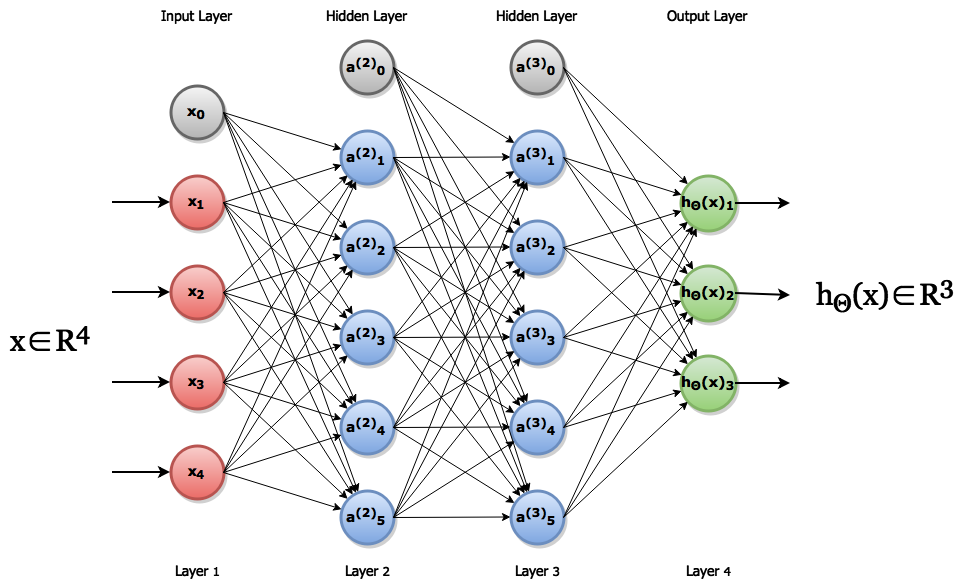
\includegraphics[width = 0.93\textwidth]{plots/neuralNetwork.png}
	\caption[An artificial neural network]{A small neural network: input layer with 4 units (red), two hidden layers of 5 units (blue) and output layer of 3 units (green). Bias units appear in gray. It approximates a function $h_\Theta(x): \mathbb{R}^4 \to \mathbb{R}^3$, i.e., it classifies an input vector $x \in \mathbb{R}^4$ into 3 possible classes.}
	\label{fig:NeuralNetwork}
\end{figure}

A unit computes a function of the form:
\begin{equation}
	a^{(l)}_i = g \left(\sum_{j=0}^{s^{(l-1)}} \Theta^{(l-1)}_{ij}a_j^{(l-1)}\right) \text{ for $l= 2,\dots,L-1$ and $i = 1,\dots,s^{(l)}$}
	\label{eq:NeuronActivation}
\end{equation}
where $a^{(l)}_i$ is the \emph{activation} or output of unit $i$ in layer $l$;
$g(\cdot)$ is an \emph{activation function} (defined below);
$s^{(l)}$ is the number of units in layer $l$;
$a^{(u)}_0 = 1$, for all $u = 1, \ldots, L-1$ (defined below);
$a^{(1)}_v = x_v$ for all $v = 1, \ldots, n$ i.e., the activation of the input layer is the input $x$;
$a^{(L)}_i = \sum_{j=0}^{s^{(L-1)}} \Theta^{(L-1)}_{ij}a_j^{(L-1)}$ for all $i = 1,\dots,s^{(L)}$ i.e., $g(\cdot)$ is omitted in the output layer
and $\Theta^{(l)} \in \mathbb{R}^{s^{l+1} \times s^{l}} $ is the matrix of weights connecting layer $l$ to $l+1$. Equation~\ref{eq:NeuronActivation} seems convoluted but it simply defines the activation of a unit as the weighted linear combination of the activations of units in the previous layer passed through a nonlinear function $g(\cdot)$. 

Each layer (except for the output layer) includes a \emph{bias unit} that outputs 1 regardless of its input ($a^{(1)}_0 = 1$, $a^{(2)}_0 = 1$, etc) allowing units in the next layer to learn a parameter $\Theta_{i 0}$ to account for its own predisposition to activate.
%~\footnote{This mechanism is rather technical and depends on the activation function.} |More technichally, they allow the y intercept of ... to be different thna 0 giving us more expressive power. 
Bias units are included in the vectors $a^{(l)}$, hence, the sumation in Equation~\ref{eq:NeuronActivation} starts at 0 instead of 1.

\begin{comment}
The activation function $g(\cdot)$ is usually a \emph{logistic sigmoid function}:
\begin{equation}
	g(z) = \frac{1}{1+ e^{-z}}
\end{equation}
The sigmoid function has range [0,1] and is differentiable with respect to $z$. Because of this characteristics it is used to represent probabilities in the logistic regression classifier. \emph{Logistic regression} for binary classification models the probability that $x \in \mathbb{R}^n$ belongs to the positive class as $g(w^Tx)$ and estimates the parameters $w \in \mathbb{R}^n$ during training. Any input whose output $g(w^Tx)$ is greater than $0.5$ is classified as positive, otherwise it is classified as negative. The sigmoid function equals $0.5$ when $w^Tx = 0$, thus, the decision boundary of a logistic regression classifier is $w^Tx = 0$, which is a linear function. 

However, the sigmoid function, per se, is not linear on its input $z$. Therefore, each unit in a neural network with sigmoid activation functions outputs a nonlinear activation $g(z)$ which in turn is received by units in the next layer, linearly recombined with the activation of other units and passed again through a sigmoid function; these operations are repeated until the input reaches the output layer. As a result, the function calculated by units in the output layer $h_\Theta(x)$ will be highly nonlinear on the original input $x$. This is the reason why neural networks can model functions which are highly nonlinear and why increasing the number of layers in a neural network increases the predictive power of the model. By the same token, it may be insightful to think of each unit in a neural network as a feature detector (via logistic regression): units in the first hidden layer are trained to activate when simple features are found on the input, units on the second hidden layer activate when a combination of these simple features is present on the input and so on. Thus, the network will learn to detect the most relevant features for the classification task and as the number of units increases, it learns ever more complex features (granted that there is enough training data).
\end{comment}

The activation function $g(\cdot)$ is usually a \emph{rectified linear unit} or \emph{ReLU}:
\begin{equation}
	g(z) = \max(0,z)
\end{equation}
This nonlinear function and its derivative ($1_{z>0}$) are computed easily and, unlike sigmoid or tanh activation functions, are inmune to vanishing and exploding gradients. Besides, it greatly accelerates convergence of gradient descent~\cite{Krizhevsky2012} and is currently the recommended activation function for deep neural networks~\cite{Karpathy2016}.

The vector of activations in the output layer $a^{(L)} \in \mathbb{R}^{s^{(L)}}$, called a \emph{score vector}, is the predicted (unnormalized log) probabilities $h_\Theta(x) \in \mathbb{R}^K$ that example $x$ belongs to class $k \in K$. We can exponentiate each of these values and normalize them to obtain a probability distribution over the possible classes $K$ ($p(x) \in [0..1]^K$); this improves interpretability and preserves original predictions.

Every unit produces a nonlinear activation $g(z)$ that is received by units in the next layer, linearly recombined with the activation of other units and passed again through the nonlinear function $g(z)$; these operations repeat until the processed input reaches the output layer. As a result, the network computes a function $h_\Theta(x)$ that is highly nonlinear on the original input $x$. This explains why neural networks are able to model complex functions and why increasing the number of layers increases its expressive power. It may be insightful to think of each unit as a feature detector: in the first hidden layer, units learn to detect simple features of the input, in the second hidden layer, units activate when a distinct combination of the simple features is found and so on. Thus, the network learns to recognize the most relevant features of the input learning more complex features as the number of units increases.

The \emph{softmax} loss function for a multiclass neural network classifier is defined as:
\begin{equation}
	L(\Theta) = -\frac{1}{m} \sum_{i=1}^m \log \left ( \frac{ e^{h_\Theta(x^{(i)})_{y^{(i)}}} }{ \sum_{j=1}^K e^{ h_\Theta (x^{(i)})_j} } \right )
\end{equation}
where $m$ is the number of examples in the training set, $h_\Theta(x)$ is the score vector, $K$ is the number of classes and $(x^{(i)},y^{(i)})$ is the $i^{th}$ example. $L(\Theta)$ is differentiable with respect to $\Theta$ but non-convex, nonetheless, gradient descent usually converges to a good estimate of $\Theta$~\cite{Ng2014}. \emph{Error backpropagation}~\cite{Linnainmaa1970, Werbos1974}, an algorithm to calculate the derivatives of the loss function with respect to $\Theta$, computes error terms in the output layer and backpropagates them layer by layer using the chain rule of calculus.

%Deep neural networks are suceptible to overfitting because they need to estimate many parameters. 
Because many parameters need to be estimated, deep neural networks are susceptible to overfitting. The simplest approach to overcome this is using regularization. Regularization for neural networks is done by performing gradient descent on the regularized loss function presented in Equation~\ref{eq:ANNRegularizedLossFunction}
\begin{equation}
	L(\Theta) = -\frac{1}{m} \sum_{i=1}^m \log \left ( \frac{ e^{h_\Theta(x^{(i)})_{y^{(i)}}} }{ \sum_{j=1}^K e^{ h_\Theta (x^{(i)})_j} } \right ) + \frac{\lambda}{2m}\sum_{l=1}^{L-1}\sum_{i=1}^{s^{(l)}}\sum_{j=1}^{s^{(l+1)}} \left(\Theta^{(l)}_{ij}\right)^2
	\label{eq:ANNRegularizedLossFunction}
\end{equation}

\emph{Dropout}~\cite{Srivastava2014} is another popular method to prevent overfitting. Each training iteration, dropout samples a different network architecture from the original network and updates only a subset of the values in $\Theta$; a unit (and its connections) is retained with some probability $p$ (usually 0.5-1), and gradient descent works on this sampled network (Fig.~\ref{fig:Dropout}). During testing all units are active but their activations are scaled by $p$ to match their expected output ($p a^{(l)}_i + (1-p) 0$). This is interpreted as training many models (with shared weights) and averaging their results at test time.

\begin{figure}[h]
	\centering
	\begin{subfigure}{0.3\textwidth}
                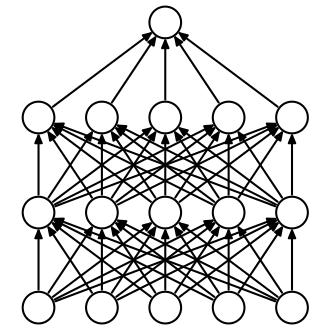
\includegraphics[width=\textwidth]{plots/dropout1.png}
		\caption{Standard neural network}
        \end{subfigure}
	~
	\begin{subfigure}{0.3\textwidth}
                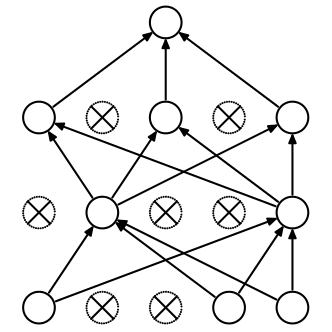
\includegraphics[width=\textwidth]{plots/dropout2.png}
		\caption{After applying dropout}
        \end{subfigure}
	\caption[Example of Dropout]{Dropout applied to a simple neural network. Crossed units are dropped. Image courtesy of~\cite{Srivastava2014}.}
	\label{fig:Dropout}
\end{figure}
